\documentclass{article}

\usepackage[round]{natbib}

\usepackage{arxiv}

\usepackage{tikz}
\usetikzlibrary{snakes,arrows,shapes}

\usepackage[utf8]{inputenc} % allow utf-8 input
\usepackage[T1]{fontenc}    % use 8-bit T1 fonts
\usepackage{hyperref}       % hyperlinks
\usepackage{url}            % simple URL typesetting
\usepackage{booktabs}       % professional-quality tables
\usepackage{amsfonts}       % blackboard math symbols
\usepackage{amsmath}
\usepackage{amsthm}
\usepackage{mathtools}
\usepackage{nicefrac}       % compact symbols for 1/2, etc.
\usepackage{microtype}      % microtypography
\newtheorem{theorem}{Theorem} %[section]
\newtheorem{lemma}{Lemma}
\newtheorem*{theorem*}{Theorem}
\theoremstyle{definition}
\newtheorem{definition}{Definition}
\newtheorem{corollary}{Corollary}

\newcommand\independent{\protect\mathpalette{\protect\independenT}{\perp}}
\def\independenT#1#2{\mathrel{\rlap{$#1#2$}\mkern2mu{#1#2}}}

\newcommand{\deq}{\stackrel{d}{=}} 

\usepackage{amssymb}

\let\oldemptyset\emptyset
\let\emptyset\varnothing


%%%%%%%%%%%%%%%%%%%%%%%%%%%%%%%%%%%%%%%%%%%%%%%%%%%%%%%%%%%%%%%%%
%%% Following part is for editing, should be commented out in the final version:
\usepackage{xcolor}
\newcommand{\todo}[1]{{\color{red}{\textbf{ToDo: #1}}}}
\usepackage{lipsum}
%%%%%%%%%%%%%%%%%%%%%%%%%%%%%%%%%%%%%%%%%%%%%%%%%%%%%%%%%%%%%%%%%


\title{A conditional permutation-based approach to test confounder effect and center-bias in machine learning models}


\author{
  Tamas~Spisak \\
  Institute for Diagnostic and Interventional Radiology and Neuroradiology \\
  University Hospital Essen\\
  Hufelandstrasse 55, 45147 Essen \\
  \texttt{tamas.spisak@uk-essen.de} \\
  %% examples of more authors
  %% \AND
  %% Coauthor \\
  %% Affiliation \\
  %% Address \\
  %% \texttt{email} \\
  %% \And
  %% Coauthor \\
  %% Affiliation \\
  %% Address \\
  %% \texttt{email} \\
  %% \And
  %% Coauthor \\
  %% Affiliation \\
  %% Address \\
  %% \texttt{email} \\
}

\begin{document}
\maketitle

\begin{abstract} % 150 words
\lipsum[1]
\end{abstract}


% keywords can be removed
\keywords{machine learning, predictive modelling, confounder, conditional independence test, conditional permutation test}


\section{Introduction}

Predictive modelling and supervised learning methods have recently became increasingly important in biomedical research and hold promise for delivering biomarkers that substantially impact clinical practice and public health \citep{kent2018personalized}. The usefulness and applicability of the such markers is to be evaluated not solely on the biomedical relevance of the predictive performance (i.e. prognostic/diagnostic value); generalizability across contexts and populations and biomedical validity (i.e. the model is driven by biomedical relevant signal) are also highly important requirements towards potential biomarkers \citep{woo2017building}.

Variables that can induce spurious associations between the predictor variables (features) and the prediction target - often referred to as confounders - can be detrimental to the model's biomedical validity and generalizability. Many types of confounders can be distinguished.
First, measurement artifacts can obviously be considered as confounders. For instance, in-scanner head motion artifacts in magnetic resonance imaging (MRI)-based predictive models can be especially problematic, if the prediction target is also associated with movement kinematics or motor function, like previously demonstrated e.g. in case of e.g Autism \citep{spisak2014voxel, spisak2019optimal} and Alzheimer's \citep{rao2017predictive}. Similarly, eye-blink artifacts can result in confound-bias in EEG-based markers \citep{eldridge2014robust}.
Second, depending on the research question, demographic and psychometric variables can also be considered as confounders during predictive modelling. E.g. resting-state functional connectivity is known to be strongly predictive to  demographic age \citep{wang2012decoding, dukart2011age} and moderately to fluid intelligence \citep{he2020deep, cole2012global}. As fluid intelligence is known to decline with aging, \citep{kievit2018neural}, models trained to predict intelligence can provide reasonable performance by simply picking up on age-related variance. 
Third, center-effects (or in general, batch effect) in multi-center studies can also cause significant bias in predictive models \citep{leek2010tackling, da2020performance}. In this case, predictive models can utilize center-effects to explain (random or true) center-differences in the predictive target. Such models will display worse-than-expected performance when applied on data from new centers.

Recently, various data harmonization approaches have been suggested to mitigate confounder-bias, ranging from simple matching \citep{rao2017predictive} or regression-based techniques \citep{rao2017predictive, dukart2011age, spisak2014voxel abdulkadir2014reduction} to the popular non-parametric empirical Bayes-based method of \cite{johnson2007adjusting} or sophisticated deep-learning oriented solutions \citep{zhao2020training, hognon2019standardization}). However, it is often unclear which variables should be considered as confounders during harmonization and considering many variables as confounder holds risks of eliminating signal-of-interest \citep{wachinger2021detect}.

Powerful statistical tests to quantify the confounding effect of certain variables in predictive models could largely foster both the the identification of confounders to correct for and the assessment of the effectiveness of various harmonization or other confound-mitigation approaches. Such methods, however, have to tackle the fact that the outputs of predictive models often have non-normal distributions (due to e.g. regularization).

Recently three dedicated techniques \citep{chaibub2019permutation, ferrari2020measuring, wachinger2021detect} have been proposed for quantifying confounder bias in predictive modelling.

The permutation-based approach of \cite{chaibub2019permutation} evaluates the null-hypothesis of no confounder bias via restricted permutations. It's p-values, however, might be invalid in certain circumstances (e.g. biased classification problems) and, as shown by \cite{ferrari2020measuring}, it does not guarantee a proper type I error control.
The 'confounder index' (CI) proposed by \cite{ferrari2020measuring}, by design, does not provide any quantification of statistical significance.
Moreover, both approaches involve repeated re-fitting of the machine learning model, which might not be feasible for models with high computational complexity (especially when hyperparameters are optimized in a nested cross-validation).
The Kolmogorov Complexity-based causal inference test, as proposed by \cite{wachinger2021detect}, aims at determining whether it is more likely that the the predictor(s) are a direct cause of the target variable or, alternatively, there exists an unobserved random variable that is the cause of both. It's computation assumes 'faithfulness' (if two variables are independent, there is no direct influence between the two in the underlying graph) a strong condition that might not be fulfilled in many real applications (e.g. functional MRI is an \emph{indirect} measure of neural activation, rendering the alternative hypothesis true in absence of any real confounder).

% todo: RO and CI: classification, KC: regression

In this paper, I formulate the 'confounder problem' as a special case of conditional independence testing. This allows relating the problem to the seminal work of \cite{shah2020hardness}, who showed that, without placing some assumptions on the joint distribution of the involved variables, establishing a conditional independence test with a valid type I error control and non-trivial power is effectively impossible ("no free lunch" theorem).

Next, I propose the conditional permutation test, a statistical test of conditional independence, recently introduced by \cite{berrett2020conditional}, as a test for evaluating confounder-bias of predictive models, based only on the target variable, the model predictions and the putative confounder.

We propose modifications to the original approach, that allow easy evaluation of the conditional distribution of $c|y$, but puts no assumptions on the distribution of the predicted values (which are often non-normal in practice).
The validity of the type I error control and the statistical power of the test is evaluated with simulated data (assuming non-normal model output).
The proposed test is then applied to provide evidence of motion-bias in the Autism Brain Imaging Data Exchange (ABIDE) dataset \citep{di2014autism} and on data from the Human Connectome Project.




\begin{itemize}
    \item growing interest in the use of
supervised learning in biomedical contexts
    \item confounder effects, site-effects
    \item approaches to deal with confounders can
    \item these approaches can eliminate signal-of-interest
    \item need for an approach that can quantify the effect of a con- founding variable and assess the effectiveness of the possible counter- measures
    \item parametric methods might fail (regularization)
    \item current solutions:
    \begin{itemize}
        \item RP: invalid p-values, continuous only with binning, involves repeating whole model training
        \item CI: no p-value, continuous only with binning, involves the whole model training
    \end{itemize}
    \item proposed method:
    \begin{itemize}
        \item based solely on the target, confounder and prediction
        \item utilizes a mathematically established non-parametric framework for testing conditional independence of the confounder and the predictions, given the observed target
        \item i.e. testing the null hypothesis that the prediction does not capture more confound than what is already present in the target variable
        \item which is usually of primary interest when investigating confounder-bias of machine learning models.
    \end{itemize}
\end{itemize}


\section{Methods}

\renewcommand{\arraystretch}{2}
\begin{table}[]
\begin{tabular}{lll}
\textbf{1.} & $y \independent \hat{y} | c$  & \quad model exclusively driven by confounder  \\
\hline
\textbf{2.} & $y \independent c | \hat{y}$ &  \quad model captures all variance in confounder \\
\hline
\textbf{3.} & $\hat{y} \independent c | y$ &   \quad model does not capture more confound than what is already given in the target variable\\
 &  
\end{tabular}
\caption{\label{tab:conditional-independence-cases} Possibilities when testing conditional independence in potentially biased predictive models. ($y$: prediction target, $\hat{y}$: predictions, $c$: confounder variable) }
\end{table}

\subsection{Notation and Background}

\begin{figure}
  \centering
  \resizebox{\columnwidth/2}{!}{%
    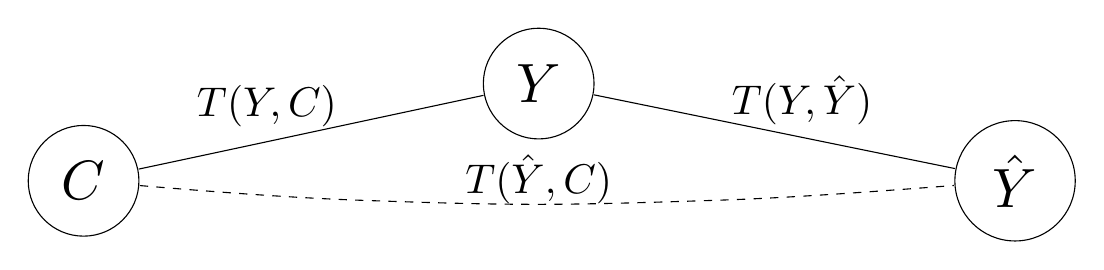
\begin{tikzpicture}[>=latex',line join=bevel,]
    %%
    \node[scale=2] (c) at (32.497bp,18.0bp) [draw,circle, minimum width=20pt] {$C$};
      \node[scale=2] (y) at (196.34bp,53.0bp) [draw,circle, minimum width=20pt] {$Y$};
      \node[scale=2] (yhat) at (367.83bp,18.0bp) [draw,circle, minimum width=20pt] {$\hat{Y}$};
      \draw [] (c) ..controls (85.995bp,29.353bp) and (118.04bp,36.283bp)  .. (y);
      \definecolor{strokecol}{rgb}{0.0,0.0,0.0};
      \pgfsetstrokecolor{strokecol}
      \draw (98.494bp,45bp) node[scale=1.5] {$T(Y,C)$};
      \draw [dashed] (c) ..controls (84.285bp,13.611bp) and (109.55bp,11.797bp)  .. (131.99bp,11.0bp) .. controls (189.15bp,8.9715bp) and (203.52bp,9.1172bp)  .. (260.68bp,11.0bp) .. controls (280.99bp,11.669bp) and (303.44bp,13.055bp)  .. (yhat);
      \draw (196.34bp,18.5bp) node[scale=1.5] {$T(\hat{Y},C)$};
      \draw [] (y) ..controls (273.69bp,37.233bp) and (303.37bp,31.105bp)  .. (yhat);
      \draw (291.18bp,47bp) node[scale=1.5] {$T(Y,\hat{Y})$};
    %
    \end{tikzpicture}
    }
  \caption{Schematic diagram of testing $\hat{y} \independent c | y$ (option 3. in Table \ref{tab:conditional-independence-cases}). $T$ is a test statistic of choice. The null hypothesis of $\hat{y} \independent c | y$ implies that $(\hat{Y}|C=c, Y=y) \deq (\hat{Y}|Y=y)$ or, equivalently $(C|\hat{Y}=\hat{y}, Y=y) \deq (C|Y=y)$.}
  \label{fig:dummy-graph}
\end{figure}



\paragraph{The conditional permutation test for independence}
 
\subsection{Conditional Permutation-based confounder-bias test}

\subsection{Validation on simulated data}

\subsection{Validation on neuroimaging data}

\section{Results}

\subsection{Simulations}

\subsection{Neuroimaging data}

\section{Discussion}

\section{Conclusion}

%\begin{figure}
%  \centering
%  \fbox{\rule[-.5cm]{4cm}{4cm} \rule[-.5cm]{4cm}{0cm}}
%  \caption{Sample figure caption.}
%  \label{fig:fig1}
%\end{figure}


\bibliographystyle{apalike}  
\bibliography{references}

\input{appendix}

\end{document}
